\PassOptionsToPackage{unicode=true}{hyperref} % options for packages loaded elsewhere
\PassOptionsToPackage{hyphens}{url}
%
\documentclass[11pt,ignorenonframetext,]{beamer}
\usepackage{pgfpages}
\setbeamertemplate{caption}[numbered]
\setbeamertemplate{caption label separator}{: }
\setbeamercolor{caption name}{fg=normal text.fg}
\beamertemplatenavigationsymbolsempty
% Prevent slide breaks in the middle of a paragraph:
\widowpenalties 1 10000
\raggedbottom
\setbeamertemplate{part page}{
\centering
\begin{beamercolorbox}[sep=16pt,center]{part title}
  \usebeamerfont{part title}\insertpart\par
\end{beamercolorbox}
}
\setbeamertemplate{section page}{
\centering
\begin{beamercolorbox}[sep=12pt,center]{part title}
  \usebeamerfont{section title}\insertsection\par
\end{beamercolorbox}
}
\setbeamertemplate{subsection page}{
\centering
\begin{beamercolorbox}[sep=8pt,center]{part title}
  \usebeamerfont{subsection title}\insertsubsection\par
\end{beamercolorbox}
}
\AtBeginPart{
  \frame{\partpage}
}
\AtBeginSection{
  \ifbibliography
  \else
    \frame{\sectionpage}
  \fi
}
\AtBeginSubsection{
  \frame{\subsectionpage}
}
\usepackage{lmodern}
\usepackage{amssymb,amsmath}
\usepackage{ifxetex,ifluatex}
\usepackage{fixltx2e} % provides \textsubscript
\ifnum 0\ifxetex 1\fi\ifluatex 1\fi=0 % if pdftex
  \usepackage[T1]{fontenc}
  \usepackage[utf8]{inputenc}
  \usepackage{textcomp} % provides euro and other symbols
\else % if luatex or xelatex
  \usepackage{unicode-math}
  \defaultfontfeatures{Ligatures=TeX,Scale=MatchLowercase}
\fi
\usetheme[]{metropolis}
% use upquote if available, for straight quotes in verbatim environments
\IfFileExists{upquote.sty}{\usepackage{upquote}}{}
% use microtype if available
\IfFileExists{microtype.sty}{%
\usepackage[]{microtype}
\UseMicrotypeSet[protrusion]{basicmath} % disable protrusion for tt fonts
}{}
\IfFileExists{parskip.sty}{%
\usepackage{parskip}
}{% else
\setlength{\parindent}{0pt}
\setlength{\parskip}{6pt plus 2pt minus 1pt}
}
\usepackage{hyperref}
\hypersetup{
            pdftitle={Lecture 22},
            pdfauthor={Colin Rundel},
            pdfborder={0 0 0},
            breaklinks=true}
\urlstyle{same}  % don't use monospace font for urls
\newif\ifbibliography
\usepackage{color}
\usepackage{fancyvrb}
\newcommand{\VerbBar}{|}
\newcommand{\VERB}{\Verb[commandchars=\\\{\}]}
\DefineVerbatimEnvironment{Highlighting}{Verbatim}{commandchars=\\\{\}}
% Add ',fontsize=\small' for more characters per line
\newenvironment{Shaded}{}{}
\newcommand{\AlertTok}[1]{\textcolor[rgb]{1.00,0.00,0.00}{\textbf{#1}}}
\newcommand{\AnnotationTok}[1]{\textcolor[rgb]{0.38,0.63,0.69}{\textbf{\textit{#1}}}}
\newcommand{\AttributeTok}[1]{\textcolor[rgb]{0.49,0.56,0.16}{#1}}
\newcommand{\BaseNTok}[1]{\textcolor[rgb]{0.25,0.63,0.44}{#1}}
\newcommand{\BuiltInTok}[1]{#1}
\newcommand{\CharTok}[1]{\textcolor[rgb]{0.25,0.44,0.63}{#1}}
\newcommand{\CommentTok}[1]{\textcolor[rgb]{0.38,0.63,0.69}{\textit{#1}}}
\newcommand{\CommentVarTok}[1]{\textcolor[rgb]{0.38,0.63,0.69}{\textbf{\textit{#1}}}}
\newcommand{\ConstantTok}[1]{\textcolor[rgb]{0.53,0.00,0.00}{#1}}
\newcommand{\ControlFlowTok}[1]{\textcolor[rgb]{0.00,0.44,0.13}{\textbf{#1}}}
\newcommand{\DataTypeTok}[1]{\textcolor[rgb]{0.56,0.13,0.00}{#1}}
\newcommand{\DecValTok}[1]{\textcolor[rgb]{0.25,0.63,0.44}{#1}}
\newcommand{\DocumentationTok}[1]{\textcolor[rgb]{0.73,0.13,0.13}{\textit{#1}}}
\newcommand{\ErrorTok}[1]{\textcolor[rgb]{1.00,0.00,0.00}{\textbf{#1}}}
\newcommand{\ExtensionTok}[1]{#1}
\newcommand{\FloatTok}[1]{\textcolor[rgb]{0.25,0.63,0.44}{#1}}
\newcommand{\FunctionTok}[1]{\textcolor[rgb]{0.02,0.16,0.49}{#1}}
\newcommand{\ImportTok}[1]{#1}
\newcommand{\InformationTok}[1]{\textcolor[rgb]{0.38,0.63,0.69}{\textbf{\textit{#1}}}}
\newcommand{\KeywordTok}[1]{\textcolor[rgb]{0.00,0.44,0.13}{\textbf{#1}}}
\newcommand{\NormalTok}[1]{#1}
\newcommand{\OperatorTok}[1]{\textcolor[rgb]{0.40,0.40,0.40}{#1}}
\newcommand{\OtherTok}[1]{\textcolor[rgb]{0.00,0.44,0.13}{#1}}
\newcommand{\PreprocessorTok}[1]{\textcolor[rgb]{0.74,0.48,0.00}{#1}}
\newcommand{\RegionMarkerTok}[1]{#1}
\newcommand{\SpecialCharTok}[1]{\textcolor[rgb]{0.25,0.44,0.63}{#1}}
\newcommand{\SpecialStringTok}[1]{\textcolor[rgb]{0.73,0.40,0.53}{#1}}
\newcommand{\StringTok}[1]{\textcolor[rgb]{0.25,0.44,0.63}{#1}}
\newcommand{\VariableTok}[1]{\textcolor[rgb]{0.10,0.09,0.49}{#1}}
\newcommand{\VerbatimStringTok}[1]{\textcolor[rgb]{0.25,0.44,0.63}{#1}}
\newcommand{\WarningTok}[1]{\textcolor[rgb]{0.38,0.63,0.69}{\textbf{\textit{#1}}}}
\setlength{\emergencystretch}{3em}  % prevent overfull lines
\providecommand{\tightlist}{%
  \setlength{\itemsep}{0pt}\setlength{\parskip}{0pt}}
\setcounter{secnumdepth}{0}

% set default figure placement to htbp
\makeatletter
\def\fps@figure{htbp}
\makeatother

\usepackage{geometry}
\usepackage{graphicx}

\usepackage{bbold}
\usepackage{lmodern}


\usepackage{url}		% produces hyperlinks

\usepackage{colortbl}	% allows for color usage in tables
\usepackage{multirow}	% allows for rows that span multiple rows in tables

\usepackage{color}          	% gives color options
\usepackage{xcolor}		% this package has a variety of color options

\usepackage{multicol}
\usepackage{textcomp}

\usepackage{setspace}
\usepackage{changepage}
\usepackage{isotope}

\singlespacing

\def\begincol{\begin{column}}
\def\endcol{\end{column}}

\def\begincols{\begin{columns}}
\def\endcols{\end{columns}}

%%%%%%%%%%%%%%%%
% Small code output
%%%%%%%%%%%%%%%%

%% change fontsize of R code

\makeatletter
\@ifundefined{Shaded}{\newenvironment{Shaded}{}{}}{}
\makeatother


\let\oldShaded\Shaded
\let\endoldShaded\endShaded
\renewenvironment{Shaded}{\footnotesize\begin{spacing}{0.9}\oldShaded}{\endoldShaded\end{spacing}}

%% change fontsize of output
\let\oldverbatim\verbatim
\let\endoldverbatim\endverbatim
\renewenvironment{verbatim}{\footnotesize\begin{spacing}{0.9}\oldverbatim}{\endoldverbatim\end{spacing}}


\newcommand{\tinyoutput}{
  \renewenvironment{Shaded}{\tiny\begin{spacing}{0.9}\oldShaded}{\endoldShaded\end{spacing}}
  \renewenvironment{verbatim}{\tiny\begin{spacing}{0.9}\oldverbatim}{\endoldverbatim\end{spacing}}
}

\newcommand{\scriptoutput}{
  \renewenvironment{Shaded}{\scriptsize\begin{spacing}{0.9}\oldShaded}{\endoldShaded\end{spacing}}
  \renewenvironment{verbatim}{\scriptsize\begin{spacing}{0.9}\oldverbatim}{\endoldverbatim\end{spacing}}
}

\newcommand{\footnoteoutput}{
  \renewenvironment{Shaded}{\footnotesize\begin{spacing}{0.9}\oldShaded}{\endoldShaded\end{spacing}}
  \renewenvironment{verbatim}{\footnotesize\begin{spacing}{0.9}\oldverbatim}{\endoldverbatim\end{spacing}}
}

%\newcommand{\verbatimfont}[1]{\renewcommand{\verbatim@font}{\ttfamily#1}}


%%%%%%%%%%%%%%%%
% Custom Colors
%%%%%%%%%%%%%%%%

\definecolor{redhl}{rgb}{0.98,0.29,0.28}
\definecolor{yellowhl}{rgb}{0.98,0.87,0.28}


\xdefinecolor{oiBlue}{rgb}{0.15, 0.35, 0.55}
\xdefinecolor{gray}{rgb}{0.5, 0.5, 0.5}
\xdefinecolor{darkGray}{rgb}{0.3, 0.3, 0.3}
\xdefinecolor{darkerGray}{rgb}{0.2, 0.2, 0.2}
\xdefinecolor{rubineRed}{rgb}{0.89,0,0.30}
\xdefinecolor{linkCol}{rgb}{0.11,0.49,0.95}	
\xdefinecolor{irishGreen}{rgb}{0,0.60,0}	
\xdefinecolor{darkturquoise}{rgb}{0.44, 0.58, 0.86}
\definecolor{lightGreen}{rgb}{0.533,0.765,0.42}
%\xdefinecolor{hlblue}{rgb}{0.051,0.65,1}
\xdefinecolor{hlblue}{rgb}{ 0.055, 0.639, 0.831}
\definecolor{light}{rgb}{.337,.608,.741}
\definecolor{dark}{rgb}{.337,.608,.741}

\definecolor{cpink}{rgb}{0.93, 0.23, 0.51}

%%%%%%%%%%%%%%%%
% Custom Commands
%%%%%%%%%%%%%%%%

% text colors
\newcommand{\red}[1]{\textit{\textcolor{rubineRed}{#1}}}
\newcommand{\orange}[1]{\textit{\textcolor{orange}{#1}}}
\newcommand{\pink}[1]{\textit{\textcolor{rubineRed!90!white!50}{#1}}}
\newcommand{\green}[1]{\textit{\textcolor{irishGreen}{#1}}}
\newcommand{\blue}[1]{\textit{\textcolor{darkturquoise}{#1}}}
\newcommand{\light}[1]{\textcolor{light}{\textbf{#1}}}
\newcommand{\dark}[1]{\textcolor{dark}{#1}}
\newcommand{\gray}[1]{\textcolor{gray}{#1}}


% mail
\newcommand{\mail}[1]{\href{mailto:#1}{\textit{\textcolor{linkCol}{#1}}}}

% highlighting: hl, hlGr, mathhl
\newcommand{\hl}[1]{\textit{\textcolor{hlblue}{#1}}}
\newcommand{\hlGr}[1]{\textit{\textcolor{lightGreen}{#1}}}
\newcommand{\hlRd}[1]{\textit{\textcolor{rubineRed}{#1}}}
\newcommand{\mathhl}[1]{\textcolor{hlblue}{\ensuremath{#1}}}
\newcommand{\hlr}[1]{\fcolorbox{redhl}{white}{$\displaystyle #1$}}
\newcommand{\hly}[1]{\fcolorbox{yellowhl}{white}{$\displaystyle #1$}}


\newcommand{\vvfill}{\vskip0pt plus 1filll}

\DeclareMathOperator*{\argmin}{arg\,min}
\DeclareMathOperator*{\argmax}{arg\,max}

\title{Lecture 22}
\providecommand{\subtitle}[1]{}
\subtitle{Spatio-temporal Models}
\author{Colin Rundel}
\date{11/28/2018}

\begin{document}
\frame{\titlepage}

\hypertarget{spatial-models-with-ar-time-dependence}{%
\section{Spatial Models with AR time
dependence}\label{spatial-models-with-ar-time-dependence}}

\begin{frame}[fragile]{Example - Weather station data}
\protect\hypertarget{example---weather-station-data}{}

\footnotesize

Based on Andrew Finley and Sudipto Banerjee's notes from
\href{http://blue.for.msu.edu/NEON/SC/}{National Ecological Observatory
Network (NEON) Applied Bayesian Regression Workshop, March 7 - 8, 2013}
\href{http://blue.for.msu.edu/NEON/SC/exercises/exercise-6/initial-exploration-spDynLM.pdf}{Module
6}

\texttt{NETemp.dat} - Monthly temperature data (Celsius) recorded across
the Northeastern US starting in January 2000.

\scriptoutput

\begin{verbatim}
## # A tibble: 34 x 27
##        x     y  elev    t_1   t_2    t_3   t_4   t_5   t_6   t_7   t_8
##    <dbl> <dbl> <int>  <dbl> <dbl>  <dbl> <dbl> <dbl> <dbl> <dbl> <dbl>
##  1 6094. 3195.   102  -6.39 -3.61  3.72   6.78 12.6   18.4  20    20.1
##  2 6245. 3262.     1  -6.28 -4.11  2.61   6.56 11.4   16.8  18.4  18.7
##  3 6157. 3484.   157 -11.1  -9.44 -0.389  3.94  9.89  15.4  17.5  17.4
##  4 6124. 3528.   176 -11.6  -9.72 -1.17   2.89  9.67  14.8  17.4  16.9
##  5 6005. 3275.   400 -12.6  -9.06 -1.61   2.56  8.56  14.3  15.9  15.8
##  6 6052. 3226.   133  -9.11 -6.39  1.22   4.94 10.9   15.9  17.3  17.6
##  7 6099. 3185.    56  -7.94 -6.06  2.06   5.56 11.1   17    18.6  18.8
##  8 6075. 3136.    59  -6.56 -3.5   3.17   6.17 11.5   17.4  19.1  19.4
##  9 6175. 3455.   160  -9.94 -8.94 -0.278  3.56  9.61  15.3  17.7  17.3
## 10 6005. 3327.   360 -12.3  -9.44 -1.5    2.94  9     14.5  17    16.9
## # ... with 24 more rows, and 16 more variables: t_9 <dbl>, t_10 <dbl>,
## #   t_11 <dbl>, t_12 <dbl>, t_13 <dbl>, t_14 <dbl>, t_15 <dbl>,
## #   t_16 <dbl>, t_17 <dbl>, t_18 <dbl>, t_19 <dbl>, t_20 <dbl>,
## #   t_21 <dbl>, t_22 <dbl>, t_23 <dbl>, t_24 <dbl>
\end{verbatim}

\end{frame}

\begin{frame}{}
\protect\hypertarget{section}{}

\begin{center}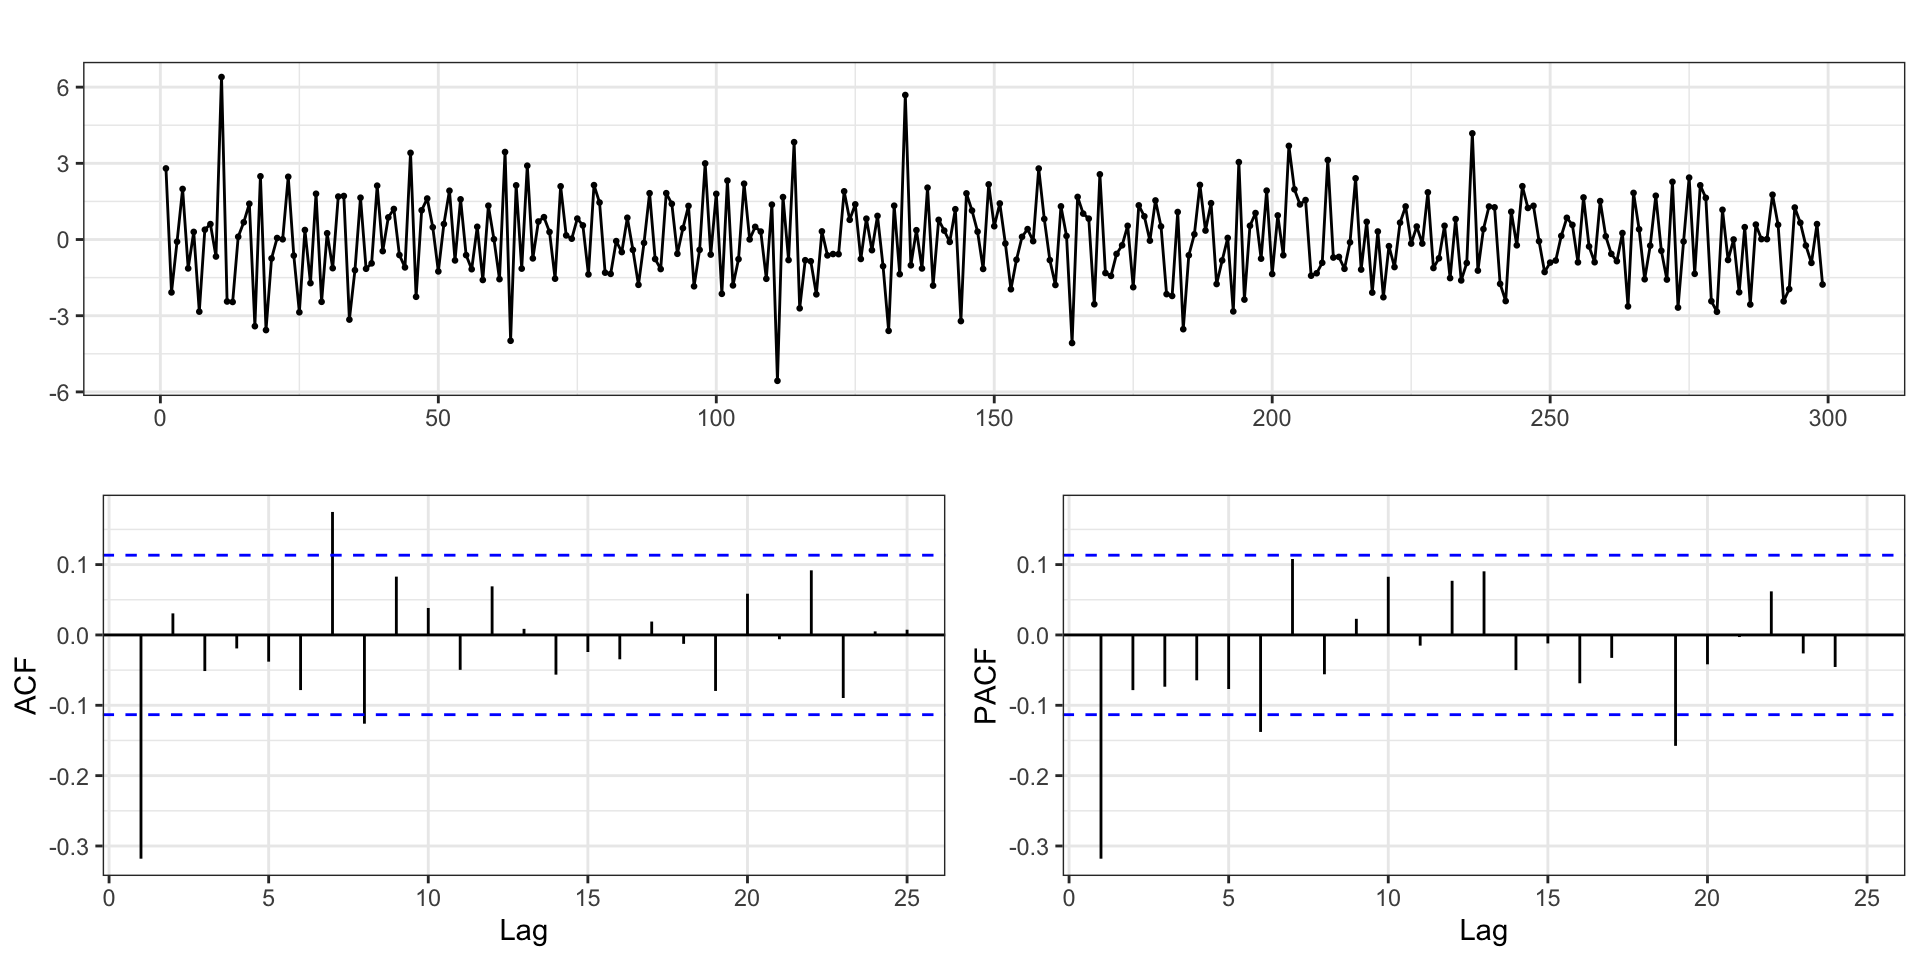
\includegraphics[width=\textwidth]{Lec22_files/figure-beamer/unnamed-chunk-2-1} \end{center}

\end{frame}

\begin{frame}{}
\protect\hypertarget{section-1}{}

\begin{center}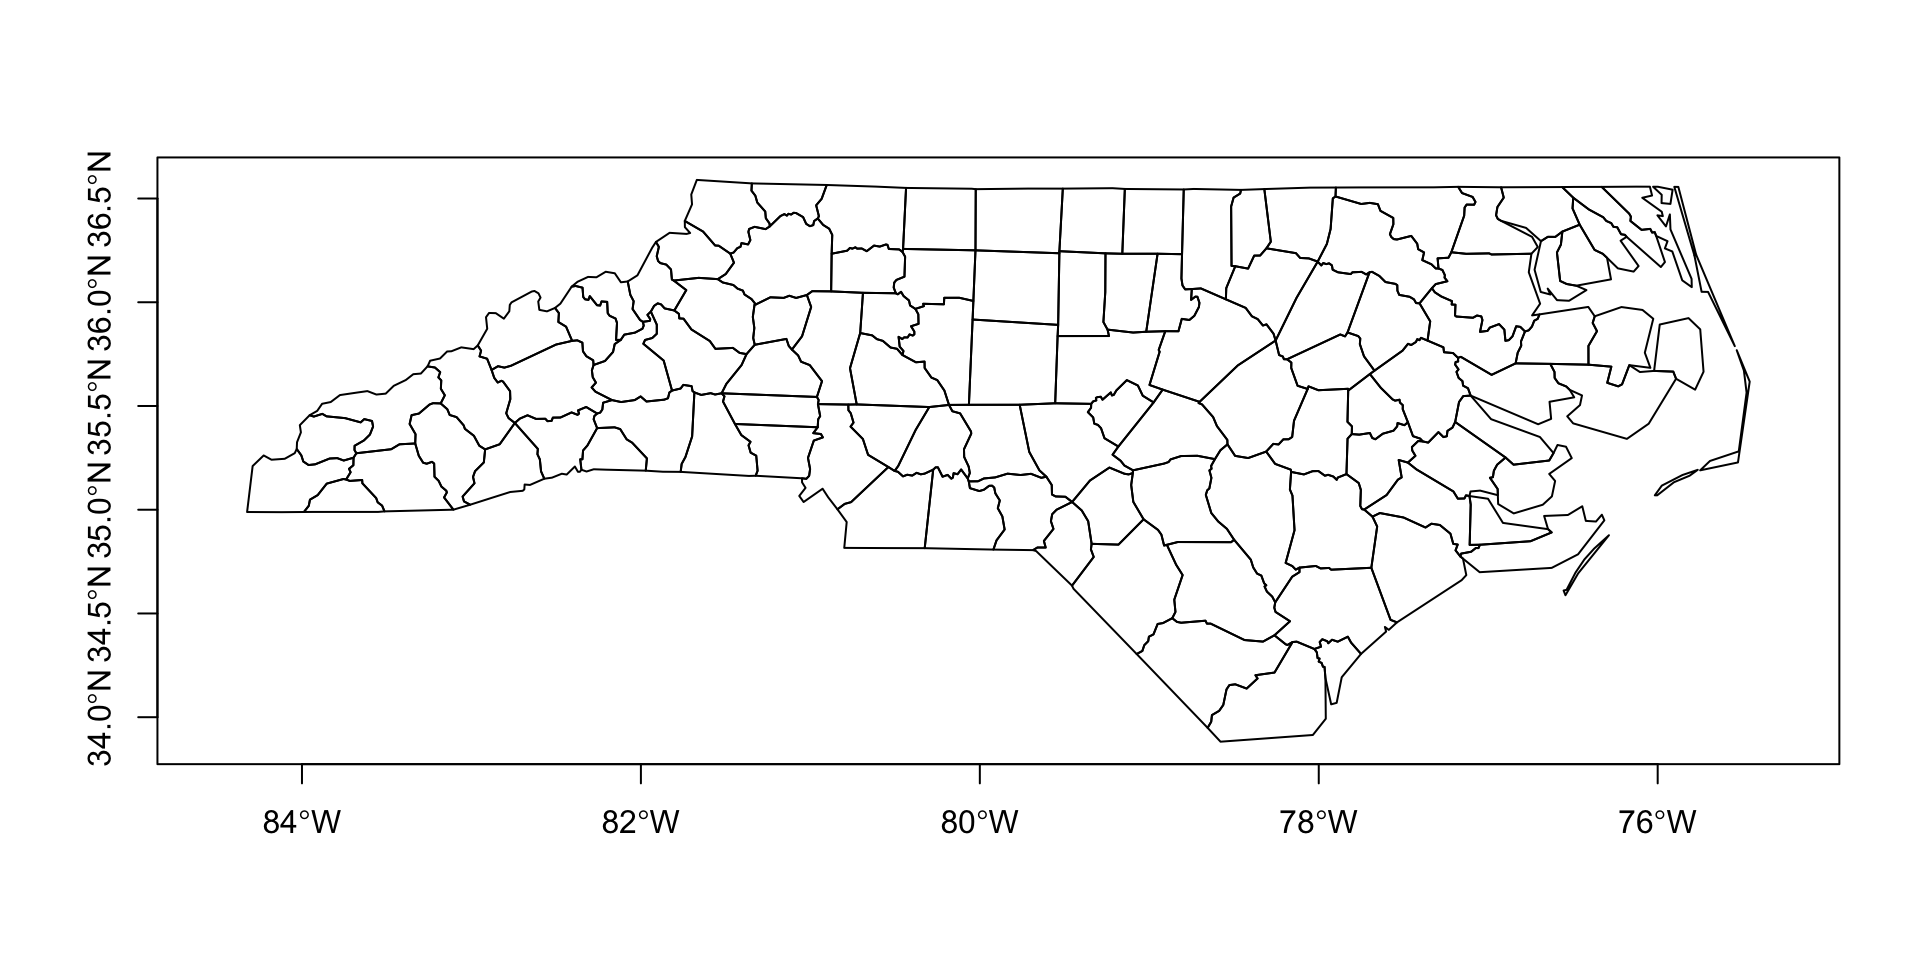
\includegraphics[width=\textwidth]{Lec22_files/figure-beamer/unnamed-chunk-3-1} \end{center}

\end{frame}

\begin{frame}{Dynamic Linear / State Space Models (time)}
\protect\hypertarget{dynamic-linear-state-space-models-time}{}

\[ 
\begin{aligned}
{{y}_t} &= \underset{1 \times p}{\symbf{F}'_t} ~ \underset{p \times 1}{\symbf{\theta}_t} + {{v}_t} 
&\qquad\qquad\text{observation equation}\\
\underset{p\times 1}{\symbf{\theta}_t} &= \underset{p \times p}{\symbf{G}_t} ~ \underset{p \times 1}{\symbf{\theta}_{t-1}}+ \underset{p \times 1}{\symbf{\omega}_t}
&\qquad\qquad\text{evolution equation}\\ 
\end{aligned}
\]

\[ 
\begin{aligned}
\symbf{v}_t &\sim \mathcal{N}(0,\symbf{V}_t) \\
\symbf{\omega}_t &\sim \mathcal{N}(0,\symbf{W}_t) \\
\end{aligned}
\]

\end{frame}

\begin{frame}[t]{DLM vs ARMA}
\protect\hypertarget{dlm-vs-arma}{}

ARMA / ARIMA are a special case of a dynamic linear model, for example
an \(AR(p)\) can be written as \[ F_t' = (1, 0, \ldots, 0) \] \[
G_t = \begin{pmatrix}
\phi_1 & \phi_2 & \cdots & \phi_{p-1} & \phi_p \\
1      & 0      & \cdots & 0          & 0      \\
0      & 1      & \cdots & 0          & 0      \\
\vdots & \vdots & \ddots & \vdots     & 0      \\
0      & 0      & \cdots & 1          & 0      \\
\end{pmatrix}
\] \[ 
\begin{aligned}
\omega_t &= (\omega_1, 0, \ldots, 0), 
\quad &\omega_1 \sim \mathcal{N}(0,\,\sigma^2)
\end{aligned}
\]

\pause

\[
\begin{aligned}
y_t &= \theta_t + v_t,
  \quad &v_t \sim \mathcal{N}(0,\, \sigma^2_v) \\
\theta_t &= \sum_{i=1}^p \phi_i\, \theta_{t-i} + \omega_1, 
  \quad &\omega_1 \sim \mathcal{N}(0,\, \sigma^2_\omega) \\
\end{aligned}
\]

\end{frame}

\begin{frame}{Dynamic spatio-temporal model}
\protect\hypertarget{dynamic-spatio-temporal-model}{}

\vspace{2mm}

The observed temperature at time \(t\) and location \(s\) is given by
\(y_t(s)\) where, \footnotesize \[
\begin{aligned}
y_t(\symbf{s}) & = \symbf{x}_t(\symbf{s})\symbf{\beta}_t + u_t(\symbf{s}) + \epsilon_t(\symbf{s}) \\
\epsilon_t(\symbf{s}) &\stackrel{ind.}\sim \mathcal{N}(0,\tau_{t}^2) \\
\\
\symbf{\beta}_t & = \symbf{\beta}_{t-1} + \symbf{\eta}_t \\
\symbf{\eta}_t &\stackrel{i.i.d.}\sim \mathcal{N}(0,\symbf{\Sigma}_{\eta}) \\
\\
u_t(\symbf{s}) &= u_{t-1}(\symbf{s}) + w_t(\symbf{s}) \\
w_t(\symbf{s}) &\stackrel{ind.}{\sim} \mathcal{N}\left(\symbf{0}, \Sigma_t(\phi_t, \sigma^2_t)\right)
\end{aligned}
\]

\vspace{3mm}

\pause

\normalsize

Additional assumptions for \(t=0\), \footnotesize \[
\symbf{\beta}_{0} \sim \mathcal{N}(\symbf{\mu}_0, \symbf{\Sigma}_0)
\] \[
u_{0}(\symbf{s}) = 0
\]

\end{frame}

\begin{frame}{Variograms by time}
\protect\hypertarget{variograms-by-time}{}

\begin{center}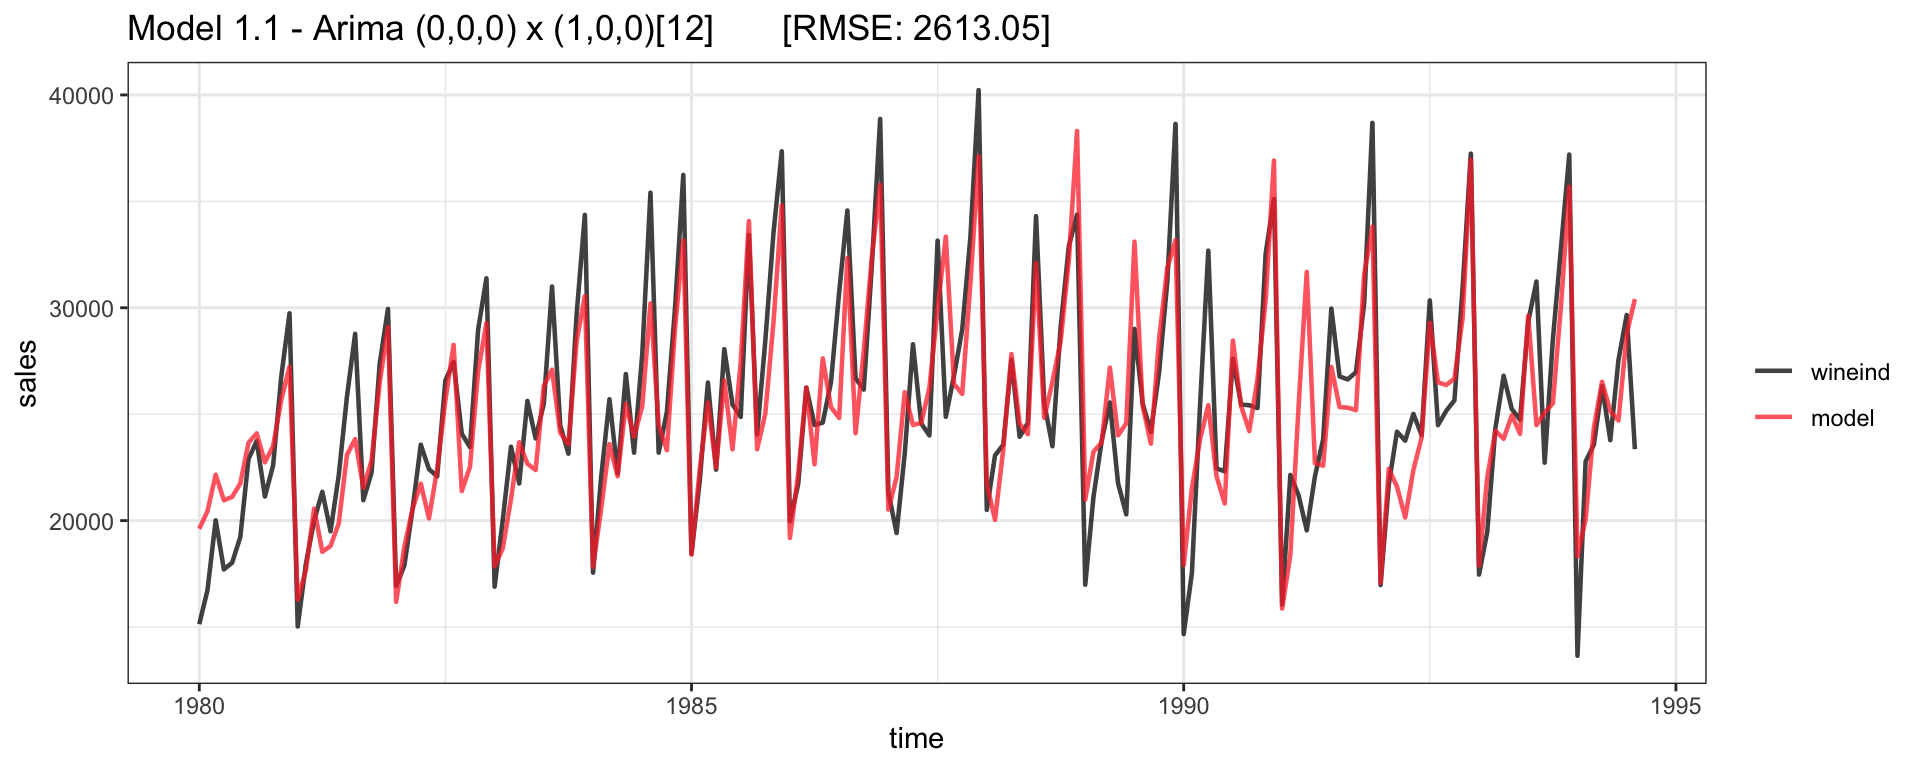
\includegraphics[width=\textwidth]{Lec22_files/figure-beamer/unnamed-chunk-4-1} \end{center}

\end{frame}

\begin{frame}[fragile]{Data and Model Parameters}
\protect\hypertarget{data-and-model-parameters}{}

\textbf{Data}: \scriptoutput

\begin{Shaded}
\begin{Highlighting}[]
\NormalTok{max_d =}\StringTok{ }\NormalTok{coords }\OperatorTok\StringTok{ }\KeywordTok{dist}\NormalTok{() }\OperatorTok\StringTok{ }\KeywordTok{max}\NormalTok{()}
\NormalTok{n_t =}\StringTok{ }\DecValTok{24}
\NormalTok{n_s =}\StringTok{ }\KeywordTok{nrow}\NormalTok{(ne_temp)}
\end{Highlighting}
\end{Shaded}

\textbf{Parameters}: \scriptoutput

\begin{Shaded}
\begin{Highlighting}[]
\NormalTok{n_beta =}\StringTok{ }\DecValTok{2}
\NormalTok{starting =}\StringTok{ }\KeywordTok{list}\NormalTok{(}
  \DataTypeTok{beta =} \KeywordTok{rep}\NormalTok{(}\DecValTok{0}\NormalTok{, n_t }\OperatorTok{*}\StringTok{ }\NormalTok{n_beta), }\DataTypeTok{phi =} \KeywordTok{rep}\NormalTok{(}\DecValTok{3}\OperatorTok{/}\NormalTok{(max_d}\OperatorTok{/}\DecValTok{4}\NormalTok{), n_t),}
  \DataTypeTok{sigma.sq =} \KeywordTok{rep}\NormalTok{(}\DecValTok{1}\NormalTok{, n_t), }\DataTypeTok{tau.sq =} \KeywordTok{rep}\NormalTok{(}\DecValTok{1}\NormalTok{, n_t), }
  \DataTypeTok{sigma.eta =} \KeywordTok{diag}\NormalTok{(}\FloatTok{0.01}\NormalTok{, n_beta)}
\NormalTok{)}
\NormalTok{tuning =}\StringTok{ }\KeywordTok{list}\NormalTok{(}\DataTypeTok{phi =} \KeywordTok{rep}\NormalTok{(}\DecValTok{1}\NormalTok{, n_t))}
\NormalTok{priors =}\StringTok{ }\KeywordTok{list}\NormalTok{(}
  \DataTypeTok{beta.0.Norm =} \KeywordTok{list}\NormalTok{(}\KeywordTok{rep}\NormalTok{(}\DecValTok{0}\NormalTok{, n_beta), }\KeywordTok{diag}\NormalTok{(}\DecValTok{1000}\NormalTok{, n_beta)), }
  \DataTypeTok{phi.Unif =} \KeywordTok{list}\NormalTok{(}\KeywordTok{rep}\NormalTok{(}\DecValTok{3}\OperatorTok{/}\NormalTok{(}\FloatTok{0.9} \OperatorTok{*}\StringTok{ }\NormalTok{max_d), n_t), }\KeywordTok{rep}\NormalTok{(}\DecValTok{3}\OperatorTok{/}\NormalTok{(}\FloatTok{0.05} \OperatorTok{*}\StringTok{ }\NormalTok{max_d), n_t)), }
  \DataTypeTok{sigma.sq.IG =} \KeywordTok{list}\NormalTok{(}\KeywordTok{rep}\NormalTok{(}\DecValTok{2}\NormalTok{, n_t), }\KeywordTok{rep}\NormalTok{(}\DecValTok{2}\NormalTok{, n_t)), }
  \DataTypeTok{tau.sq.IG =} \KeywordTok{list}\NormalTok{(}\KeywordTok{rep}\NormalTok{(}\DecValTok{2}\NormalTok{, n_t), }\KeywordTok{rep}\NormalTok{(}\DecValTok{2}\NormalTok{, n_t)),}
  \DataTypeTok{sigma.eta.IW =} \KeywordTok{list}\NormalTok{(}\DecValTok{2}\NormalTok{, }\KeywordTok{diag}\NormalTok{(}\FloatTok{0.001}\NormalTok{, n_beta))}
\NormalTok{)}
\end{Highlighting}
\end{Shaded}

\end{frame}

\begin{frame}[fragile]{Fitting with \texttt{spDynLM} from
\texttt{spBayes}}
\protect\hypertarget{fitting-with-spdynlm-from-spbayes}{}

\scriptoutput

\begin{Shaded}
\begin{Highlighting}[]
\NormalTok{n_samples =}\StringTok{ }\DecValTok{10000}
\NormalTok{models =}\StringTok{ }\KeywordTok{lapply}\NormalTok{(}\KeywordTok{paste0}\NormalTok{(}\StringTok{"t_"}\NormalTok{,}\DecValTok{1}\OperatorTok{:}\DecValTok{24}\NormalTok{, }\StringTok{"~elev"}\NormalTok{), as.formula)}

\NormalTok{m =}\StringTok{ }\NormalTok{spBayes}\OperatorTok{::}\KeywordTok{spDynLM}\NormalTok{(}
\NormalTok{  models, }\DataTypeTok{data =}\NormalTok{ ne_temp, }\DataTypeTok{coords =}\NormalTok{ coords, }\DataTypeTok{get.fitted =} \OtherTok{TRUE}\NormalTok{,}
  \DataTypeTok{starting =}\NormalTok{ starting, }\DataTypeTok{tuning =}\NormalTok{ tuning, }\DataTypeTok{priors =}\NormalTok{ priors,}
  \DataTypeTok{cov.model =} \StringTok{"exponential"}\NormalTok{, }\DataTypeTok{n.samples =}\NormalTok{ n_samples, }\DataTypeTok{n.report =} \DecValTok{1000}\NormalTok{)}

\NormalTok{m =}\StringTok{ }\KeywordTok{clean_spdynlm}\NormalTok{(m, n_samples}\OperatorTok{/}\DecValTok{2}\OperatorTok{+}\DecValTok{1}\NormalTok{, n_samples, (n_samples}\OperatorTok{/}\DecValTok{2}\NormalTok{)}\OperatorTok{/}\DecValTok{1000}\NormalTok{)}
\KeywordTok{save}\NormalTok{(m, }\DataTypeTok{file=}\StringTok{"dynlm.Rdata"}\NormalTok{)}

\CommentTok{##  ----------------------------------------}
\CommentTok{##      General model description}
\CommentTok{##  ----------------------------------------}
\CommentTok{##  Model fit with 34 observations in 24 time steps.}
\CommentTok{##  }
\CommentTok{##  Number of missing observations 0.}
\CommentTok{##  }
\CommentTok{##  Number of covariates 2 (including intercept if specified).}
\CommentTok{##  }
\CommentTok{##  Using the exponential spatial correlation model.}
\CommentTok{##  }
\CommentTok{##  Number of MCMC samples 10000.}
\CommentTok{##}
\CommentTok{##  ...}
\end{Highlighting}
\end{Shaded}

\end{frame}

\begin{frame}{Posterior Inference - \(\beta\)s}
\protect\hypertarget{posterior-inference---betas}{}

\vspace{4mm}

\begin{center}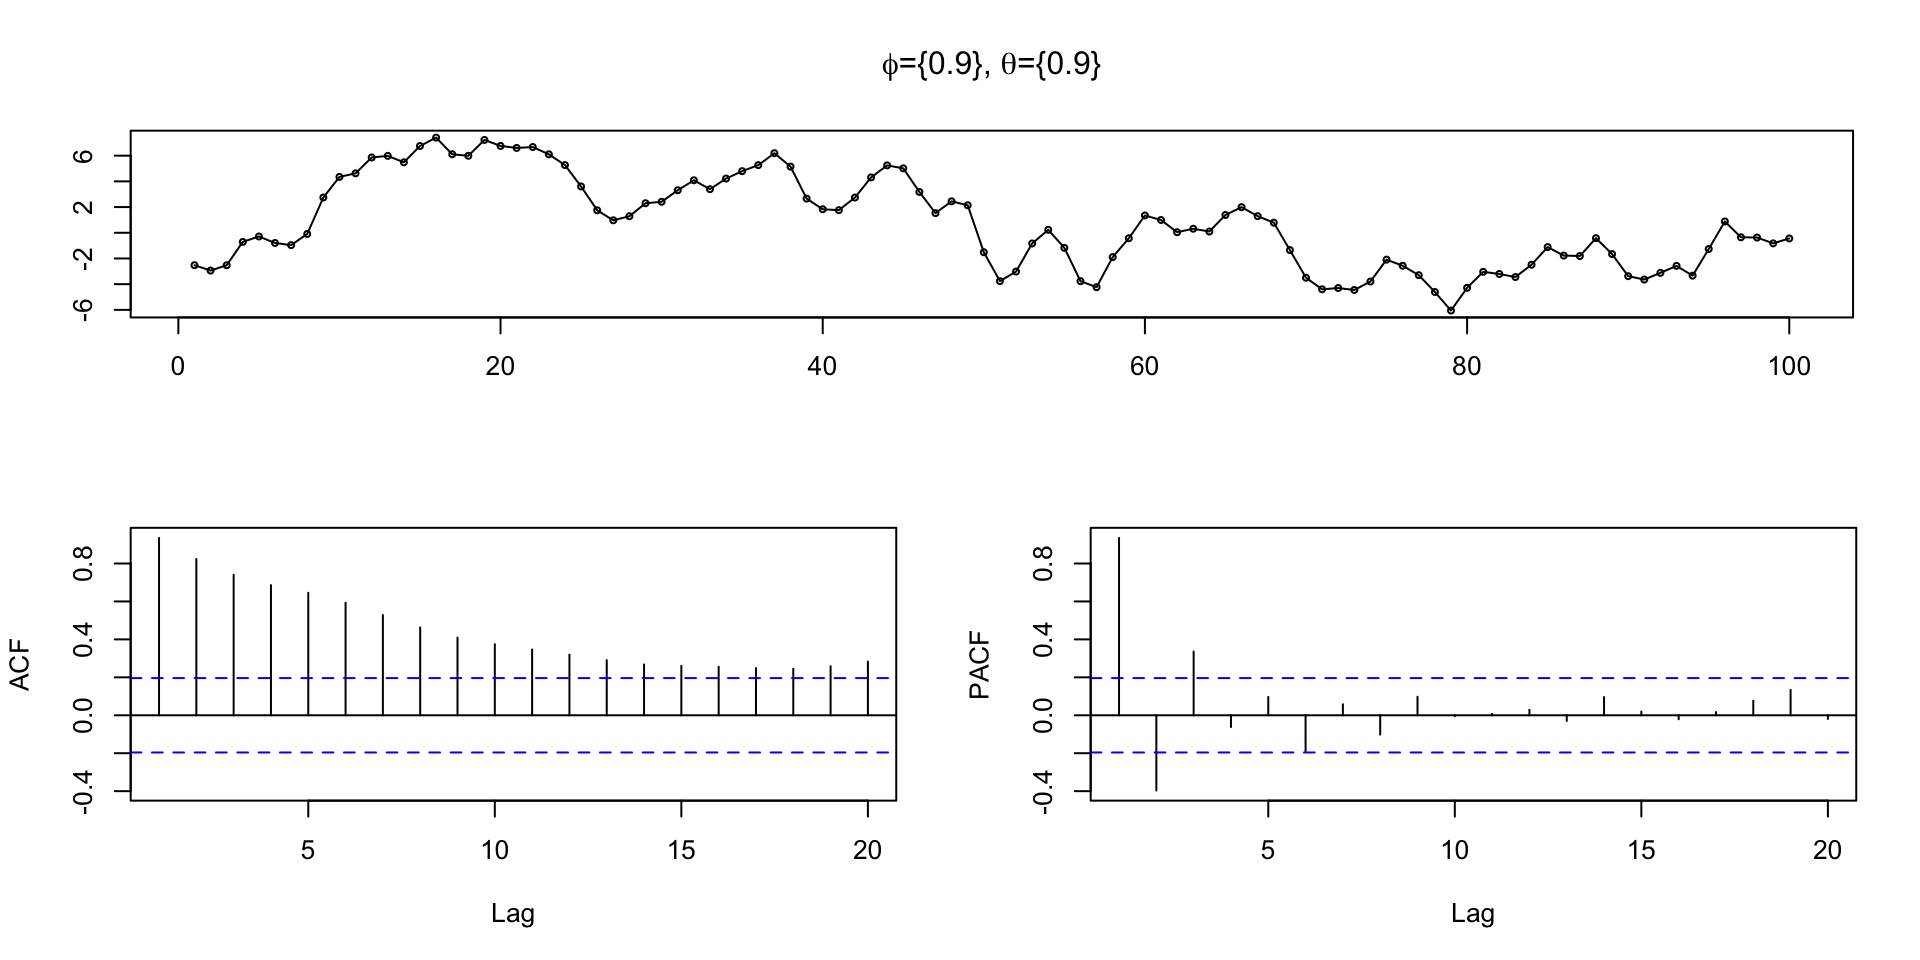
\includegraphics[width=\textwidth]{Lec22_files/figure-beamer/unnamed-chunk-9-1} \end{center}

\vvfill

\href{https://en.wikipedia.org/wiki/Lapse_rate}{Lapse Rate}
\(\approx -9.8~^\circ C/km\).

\end{frame}

\begin{frame}{Posterior Inference - \(\theta\)}
\protect\hypertarget{posterior-inference---theta}{}

\vspace{4mm}

\begin{center}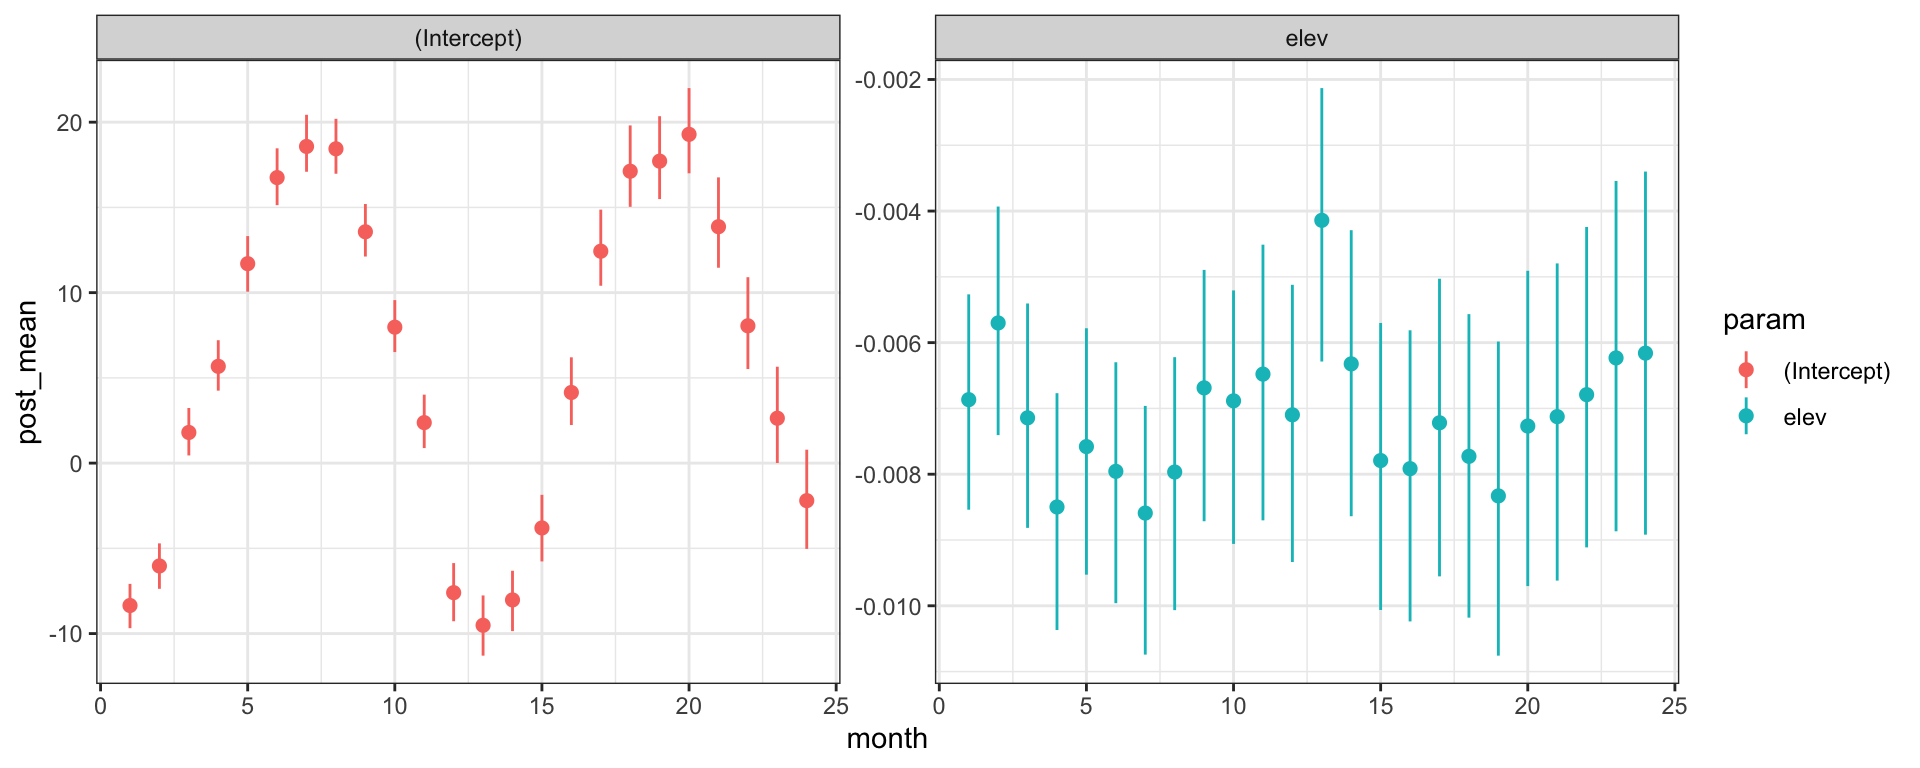
\includegraphics[width=\textwidth]{Lec22_files/figure-beamer/unnamed-chunk-10-1} \end{center}

\end{frame}

\begin{frame}{Posterior Inference - Observed vs.~Predicted}
\protect\hypertarget{posterior-inference---observed-vs.predicted}{}

\vspace{4mm}

\begin{center}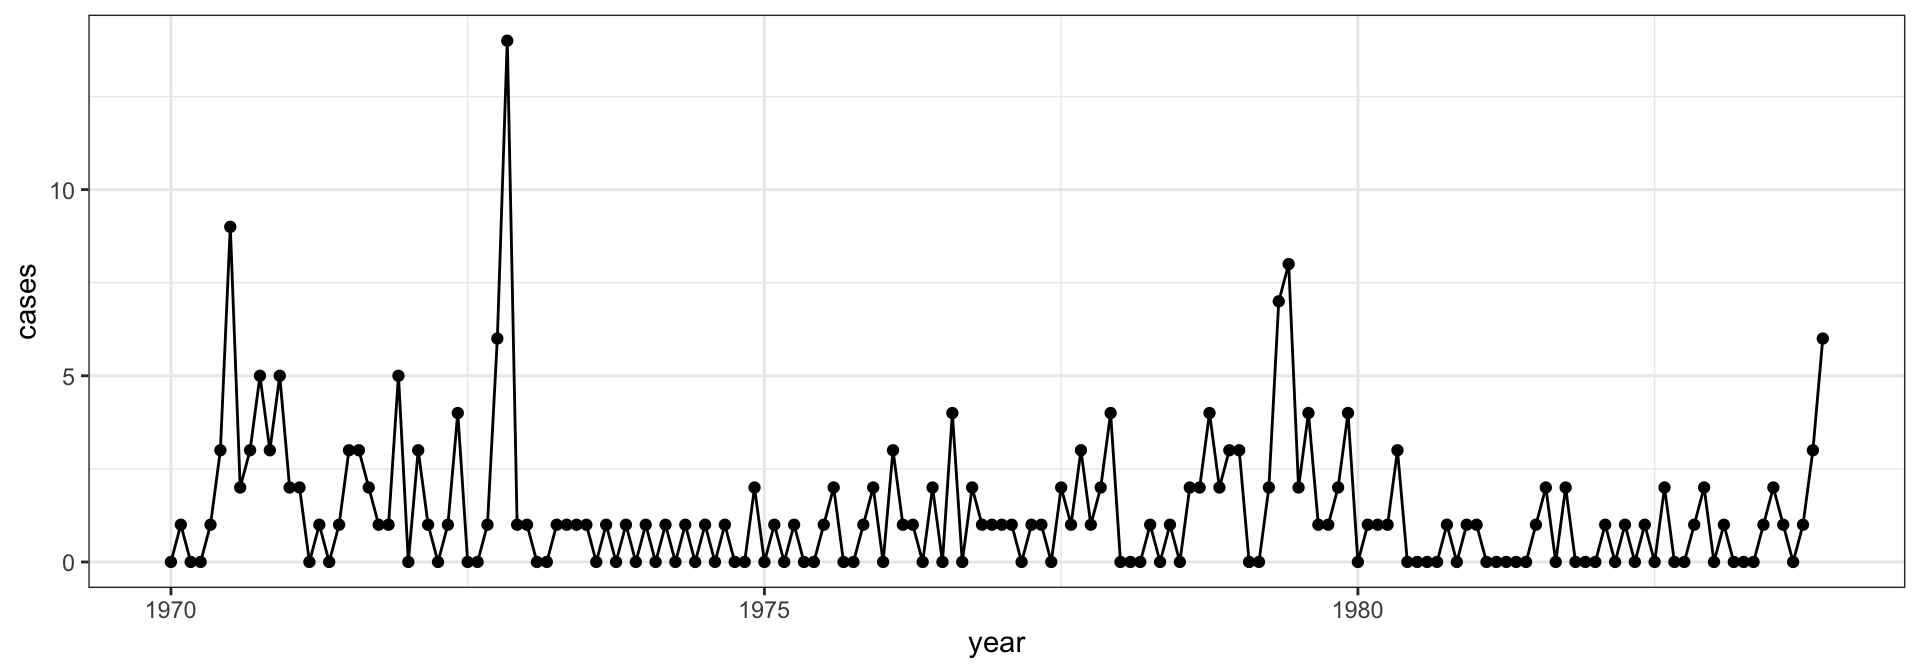
\includegraphics[width=\textwidth]{Lec22_files/figure-beamer/unnamed-chunk-11-1} \end{center}

\end{frame}

\begin{frame}[fragile]{Prediction}
\protect\hypertarget{prediction}{}

\texttt{spPredict} does not support \texttt{spDynLM} objects but it will
impute missing values.

\begin{Shaded}
\begin{Highlighting}[]
\NormalTok{r =}\StringTok{ }\KeywordTok{raster}\NormalTok{(}\DataTypeTok{xmn=}\DecValTok{5750}\NormalTok{, }\DataTypeTok{xmx=}\DecValTok{6300}\NormalTok{, }\DataTypeTok{ymn=}\DecValTok{3000}\NormalTok{, }\DataTypeTok{ymx=}\DecValTok{3550}\NormalTok{, }\DataTypeTok{nrow=}\DecValTok{20}\NormalTok{, }\DataTypeTok{ncol=}\DecValTok{20}\NormalTok{)}

\NormalTok{pred =}\StringTok{ }\KeywordTok{xyFromCell}\NormalTok{(r, }\DecValTok{1}\OperatorTok{:}\KeywordTok{length}\NormalTok{(r)) }\OperatorTok\StringTok{ }
\StringTok{  }\KeywordTok{as.data.frame}\NormalTok{() }\OperatorTok
\StringTok{  }\KeywordTok{mutate}\NormalTok{(}\DataTypeTok{type=}\StringTok{"pred"}\NormalTok{) }\OperatorTok
\StringTok{  }\KeywordTok{bind_rows}\NormalTok{(}
\NormalTok{    ne_temp }\OperatorTok\StringTok{ }\KeywordTok{mutate}\NormalTok{(}\DataTypeTok{type =} \StringTok{"obs"}\NormalTok{),}
\NormalTok{    .}
\NormalTok{  )}
\end{Highlighting}
\end{Shaded}

\end{frame}

\begin{frame}[fragile]{}
\protect\hypertarget{section-2}{}

\begin{Shaded}
\begin{Highlighting}[]
\NormalTok{models_pred =}\StringTok{ }\KeywordTok{lapply}\NormalTok{(}\KeywordTok{paste0}\NormalTok{(}\StringTok{"t_"}\NormalTok{,}\DecValTok{1}\OperatorTok{:}\NormalTok{n_t, }\StringTok{"~1"}\NormalTok{), as.formula)}

\NormalTok{n_samples =}\StringTok{ }\DecValTok{5000}
\NormalTok{m_pred =}\StringTok{ }\NormalTok{spBayes}\OperatorTok{::}\KeywordTok{spDynLM}\NormalTok{(}
\NormalTok{  models_pred, }\DataTypeTok{data =}\NormalTok{ pred, }\DataTypeTok{coords =}\NormalTok{ coords_pred, }\DataTypeTok{get.fitted =} \OtherTok{TRUE}\NormalTok{,}
  \DataTypeTok{starting =}\NormalTok{ starting, }\DataTypeTok{tuning =}\NormalTok{ tuning, }\DataTypeTok{priors =}\NormalTok{ priors,}
  \DataTypeTok{cov.model =} \StringTok{"exponential"}\NormalTok{, }\DataTypeTok{n.samples =}\NormalTok{ n_samples, }\DataTypeTok{n.report =} \DecValTok{1000}\NormalTok{)}

\NormalTok{m_pred =}\StringTok{ }\KeywordTok{clean_spdynlm}\NormalTok{(m_pred, n_samples}\OperatorTok{/}\DecValTok{2}\OperatorTok{+}\DecValTok{1}\NormalTok{, n_samples, }\DataTypeTok{thin =} \DecValTok{5}\NormalTok{)}
\KeywordTok{save}\NormalTok{(m_pred, }\DataTypeTok{file=}\StringTok{"dynlm_pred.Rdata"}\NormalTok{)}

\CommentTok{## ----------------------------------------}
\CommentTok{##  General model description}
\CommentTok{## ----------------------------------------}
\CommentTok{## Model fit with 434 observations in 24 time steps.}
\CommentTok{## }
\CommentTok{## Number of missing observations 9600.}
\CommentTok{## }
\CommentTok{## Number of covariates 1 (including intercept if specified).}
\CommentTok{## }
\CommentTok{## Using the exponential spatial correlation model.}
\CommentTok{## }
\CommentTok{## Number of MCMC samples 5000.}
\end{Highlighting}
\end{Shaded}

\end{frame}

\begin{frame}{}
\protect\hypertarget{section-3}{}

\begin{center}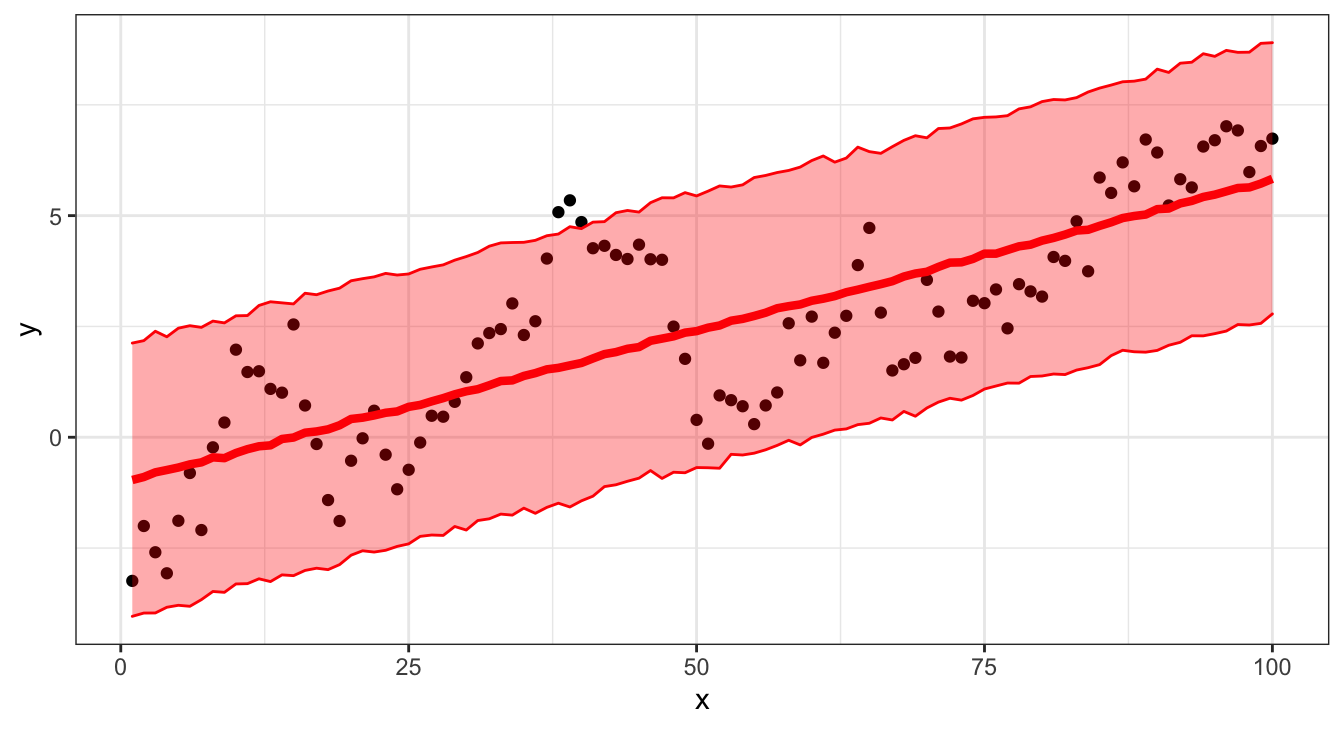
\includegraphics[width=\textwidth]{Lec22_files/figure-beamer/unnamed-chunk-16-1} \end{center}

\end{frame}

\begin{frame}{}
\protect\hypertarget{section-4}{}

\begin{center}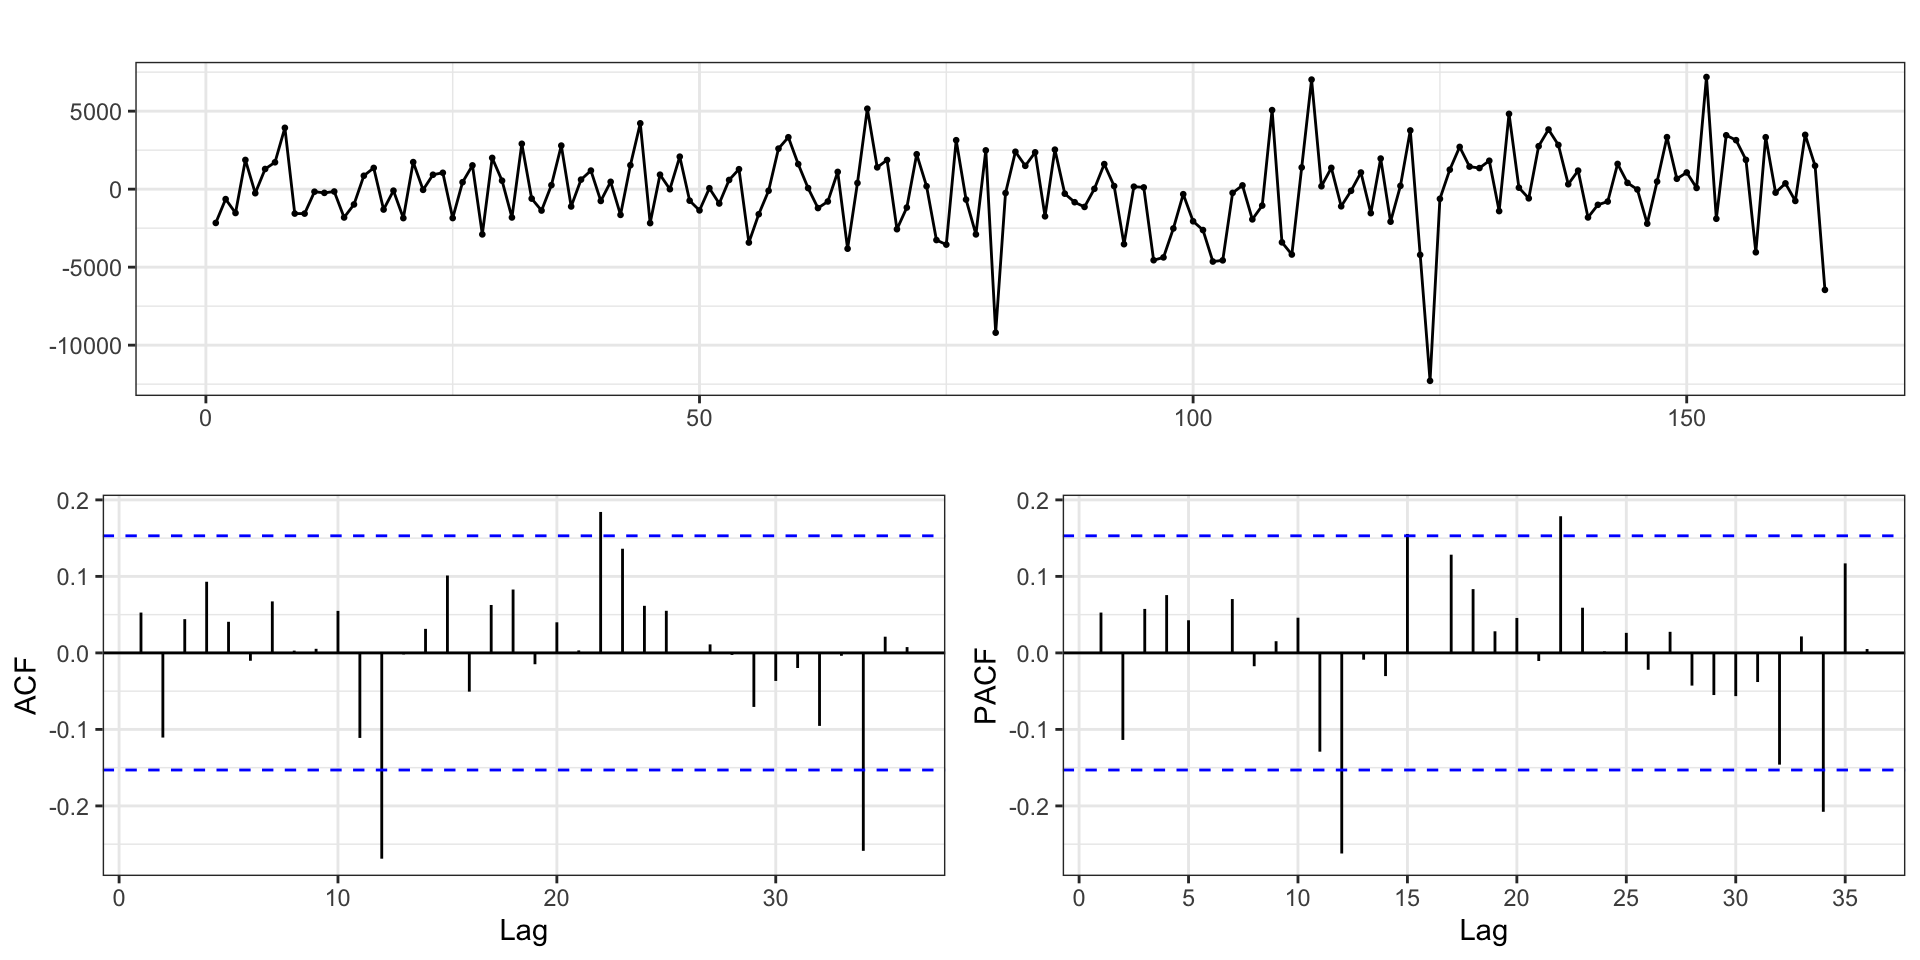
\includegraphics[width=0.8\textwidth]{Lec22_files/figure-beamer/unnamed-chunk-17-1} \end{center}

\end{frame}

\begin{frame}[fragile]{Out-of-sample validation}
\protect\hypertarget{out-of-sample-validation}{}

\begin{verbatim}
## # A tibble: 34 x 29
##        x     y  elev type  station    t_1  t_10   t_11   t_12   t_13   t_14
##    <dbl> <dbl> <int> <chr>   <int>  <dbl> <dbl>  <dbl>  <dbl>  <dbl>  <dbl>
##  1 6094. 3195.   102 test        1  NA    NA    NA      NA     NA     NA   
##  2 6245. 3262.     1 train       2  -6.28  8.89  3.89   -4.22  -7.11  -5.06
##  3 6157. 3484.   157 train       3 -11.1   6.44  1.94   -8.72 -11.6  -10.4 
##  4 6124. 3528.   176 train       4 -11.6   5.94  1.67   -9.17 -11.8  -11   
##  5 6005. 3275.   400 train       5 -12.6   5.67  0.278 -10.7  -11.9  -11   
##  6 6052. 3226.   133 train       6  -9.11  7.56  2.44   -7.11  -9.44  -8.61
##  7 6099. 3185.    56 test        7  NA    NA    NA      NA     NA     NA   
##  8 6075. 3136.    59 train       8  -6.56  9.61  4.17   -4.89  -6.06  -5.06
##  9 6175. 3455.   160 train       9  -9.94  6.67  1.72   -8.44 -12.1  -10.7 
## 10 6005. 3327.   360 train      10 -12.3   6.39  0.944 -10.6  -11.6  -10.9 
## # ... with 24 more rows, and 18 more variables: t_15 <dbl>, t_16 <dbl>,
## #   t_17 <dbl>, t_18 <dbl>, t_19 <dbl>, t_2 <dbl>, t_20 <dbl>, t_21 <dbl>,
## #   t_22 <dbl>, t_23 <dbl>, t_24 <dbl>, t_3 <dbl>, t_4 <dbl>, t_5 <dbl>,
## #   t_6 <dbl>, t_7 <dbl>, t_8 <dbl>, t_9 <dbl>
\end{verbatim}

\end{frame}

\begin{frame}{}
\protect\hypertarget{section-5}{}

\begin{center}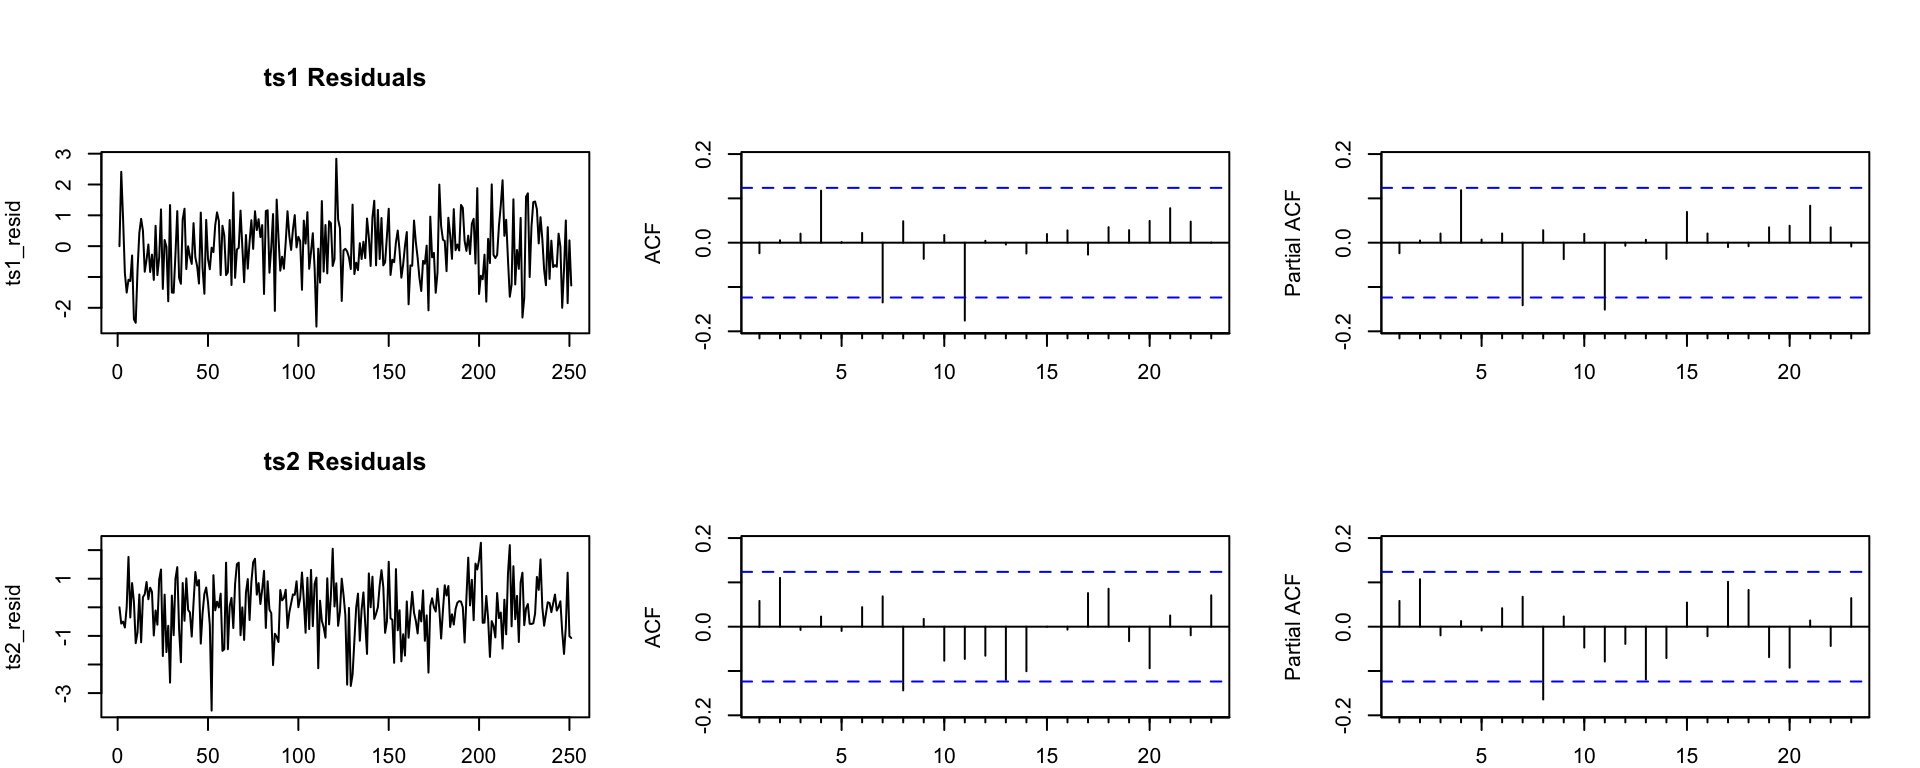
\includegraphics[width=\textwidth]{Lec22_files/figure-beamer/unnamed-chunk-21-1} \end{center}

\end{frame}

\hypertarget{spatio-temporal-models-for-continuous-time}{%
\section{Spatio-temporal models for continuous
time}\label{spatio-temporal-models-for-continuous-time}}

\begin{frame}[t]{Additive Models}
\protect\hypertarget{additive-models}{}

In general, spatiotemporal models will have a form like the following,

\[
\begin{aligned}
y(\symbf{s},{t}) 
  &= \underset{\text{mean structure}}{\mu(\symbf{s},{t})} + \underset{\text{error structure}}{{e}(\symbf{s},{t})} \\
  &= \underset{\text{Regression}}{\symbf{x}(\symbf{s},{t}) \, \symbf{\beta}(\symbf{s},{t})} + \underset{\text{Spatiotemporal RE}}{{w}(\symbf{s},{t})} + \underset{\text{White Noise}}{\epsilon(\symbf{s},{t})}
\end{aligned} 
\]

\pause

\vspace{5mm}

The simplest possible spatiotemporal model is one were assume there is
no dependence between observations in space and time,

\[
w(\symbf{s},t) = \alpha(t) + \omega(\symbf{s})
\]

these are straight forward to fit and interpret but are quite limiting
(no shared information between space and time).

\end{frame}

\begin{frame}{Spatiotemporal Covariance}
\protect\hypertarget{spatiotemporal-covariance}{}

Lets assume that we want to define our spatiotemporal random effect to
be a single stationary Gaussian Process (in 3 dimensions\(^\star\)), \[ 
\symbf{w}(\symbf{s},\symbf{t}) \sim \mathcal{N}\big(\symbf{0}, \symbf{\Sigma}(\symbf{s},\symbf{t})\big) 
\] where our covariance function depends on both \(\lVert s-s'\rVert\)
and \(\lvert t-t'\rvert\), \[
\text{cov}(\symbf{w}(\symbf{s},\symbf{t}), \symbf{w}(\symbf{s}',\symbf{t}')) = c(\lVert s-s'\rVert, \lvert t-t'\rvert)
\]

\pause

\begin{itemize}
\item
  Note that the resulting covariance matrix \(\Sigma\) will be of size
  \(n_s \cdot n_t \times n_s \cdot n_t\).

  \begin{itemize}
  \item
    Even for modest problems this gets very large (past the point of
    direct computability).
  \item
    If \(n_t = 52\) and \(n_s = 100\) we have to work with a
    \(5200 \times 5200\) covariance matrix
  \end{itemize}
\end{itemize}

\end{frame}

\begin{frame}{Separable Models}
\protect\hypertarget{separable-models}{}

One solution is to use a seperable form, where the covariance is the
product of a valid 2d spatial and a valid 1d temporal covariance /
correlation function, \[
\text{cov}(\symbf{w}(\symbf{s},\symbf{t}), \symbf{w}(\symbf{s}',\symbf{t}')) = \sigma^2 \, \rho_1(\lVert \symbf{s}-\symbf{s}'\rVert;\symbf{\theta}) \, \rho_2(\lvert \symbf{t}-\symbf{t}' \rvert; \symbf{\phi})
\] \pause If we define our observations as follows (stacking time
locations within spatial locations) \footnotesize \[
\symbf{w}(\symbf{s},\symbf{t}) = \big(
  w(\symbf{s}_1,t_1)     ,\, \cdots ,\, w(\symbf{s}_1,t_{n_t}) ,\,
  \cdots ,\,
  w(\symbf{s}_{n_s},t_1) ,\, \cdots ,\, w(\symbf{s}_{n_s},t_{n_t}) \big)^t
\] \normalsize then the covariance can be written as \footnotesize \[
\underset{n_s n_t \,\times\, n_s n_t}{\symbf{\Sigma}_w(\sigma^2, \theta, \phi)} = \sigma^2 \, \underset{n_s \,\times\, n_s}{\symbf{H}_s(\theta)} \otimes \underset{n_t \,\times\, n_t}{\symbf{H}_t(\phi)}
\] \normalsize where \(\symbf{H}_s(\theta)\) and \(\symbf{H}_t(\theta)\)
are correlation matrices defined by \footnotesize \[
\begin{aligned}
\{\symbf{H}_s(\theta)\}_{ij} &= \rho_1(\lVert \symbf{s}_i - \symbf{s}_j \rVert; \theta) \\
\{\symbf{H}_t(\phi)\}_{ij} &= \rho_2(\lvert t_i - t_j \rvert; \phi) \\
\end{aligned}
\]

\end{frame}

\begin{frame}{Kronecker Product}
\protect\hypertarget{kronecker-product}{}

Definition: \[
\begin{aligned}
\underset{[m \times n]}{\symbf{A}} \otimes \underset{[p \times q]}{\symbf{B}} = \underset{[m \cdot p \times  n \cdot q]}{\begin{pmatrix}
a_{11} \symbf{B} & \cdots & a_{1n} \symbf{B} \\
\vdots        & \ddots & \vdots        \\
a_{m1} \symbf{B} & \cdots & a_{mn} \symbf{B} \\
\end{pmatrix}}
\end{aligned}
\]

\vspace{4mm}

\pause

Properties: \[
\begin{aligned}
\symbf{A} \otimes \symbf{B}       &\ne \symbf{B} \otimes \symbf{A}  \qquad\text{(usually)} \\ 
(\symbf{A} \otimes \symbf{B})^t   &= \symbf{A}^t \otimes \symbf{B}^t \\ \\
\det(\symbf{A} \otimes \symbf{B}) &= \det(\symbf{B} \otimes \symbf{A}) \\ 
&=\det(\symbf{A})^{\text{rank}(\symbf{B})} \det(\symbf{B})^{\text{rank}(\symbf{A})} \\ \\
(\symbf{A} \otimes \symbf{B})^{-1} &= \symbf{A}^{-1} \symbf{B}^{-1}
\end{aligned}
\]

\end{frame}

\begin{frame}{Kronecker Product and MVN Likelihoods}
\protect\hypertarget{kronecker-product-and-mvn-likelihoods}{}

If we have a spatiotemporal random effect with a separable form, \[
\symbf{w}(\symbf{s},\symbf{t}) \sim \mathcal{N}(\symbf{0},\, \symbf{\Sigma}_w)
\] \[
\symbf{\Sigma}_w = \sigma^2 \, \symbf{H}_s \otimes \symbf{H}_t
\]

then the likelihood for \(\symbf{w}\) is given by

\[
-\frac{n}{2}\log 2\pi - \frac{1}{2} \log |\Sigma_w| - \frac{1}{2} \symbf{w}^t \symbf{\Sigma_w}^{-1} \symbf{w}
\] \[
= -\frac{n}{2}\log 2\pi - \frac{1}{2} \log \left[ (\sigma^2)^{n_t \cdot n_s} |H_s|^{n_t} |H_t|^{n_s}\right] - \frac{1}{2\sigma^2} \symbf{w}^t (\symbf{H}_s^{-1} \otimes \symbf{H}_t^{-1}) \symbf{w}
\]

\end{frame}

\begin{frame}[t]{Non-seperable Models}
\protect\hypertarget{non-seperable-models}{}

\begin{itemize}
\tightlist
\item
  Additive and separable models are still somewhat limiting
\end{itemize}

\vspace{2mm}

\begin{itemize}
\tightlist
\item
  Cannot treat spatiotemporal covariances as 3d observations
\end{itemize}

\vspace{2mm}

\begin{itemize}
\item
  Possible alternatives:

  \begin{itemize}
  \item
    Specialized spatiotemporal covariance functions, i.e.~\[ 
    \gamma(\symbf{s},\symbf{s}', t,t') 
    = \sigma^2 (\lvert t - t'\rvert+1)^{-1} \exp\big(-\lVert\symbf{s}-\symbf{s}'\rVert (\lvert t-t' \rvert + 1)^{-\beta/2}\big)
    \]
  \item
    Mixtures of separable covariances, i.e.~\[
    w(\symbf{s},t) = w_1(\symbf{s},t) + w_2(\symbf{s},t)
    \]
  \end{itemize}
\end{itemize}

\end{frame}

\end{document}
